\par Voici le plan qui est utilisé pour rédiger au sujet du site d'étude.
\begin{itemize}
   \item Brève présentation du pont Jacques-Cartier, et de la piste multifonctionnelle;
   \item Présentation des difficultés de l'usage de la piste l'hiver et des défis et raisons (technique, politique, sécurité) de pouvoir la conserver ouverte toute l'année, en lien avec les objectifs de l'essai 
\end{itemize}
\label{carte_site_etude}
\begin{figure}
    \centering
    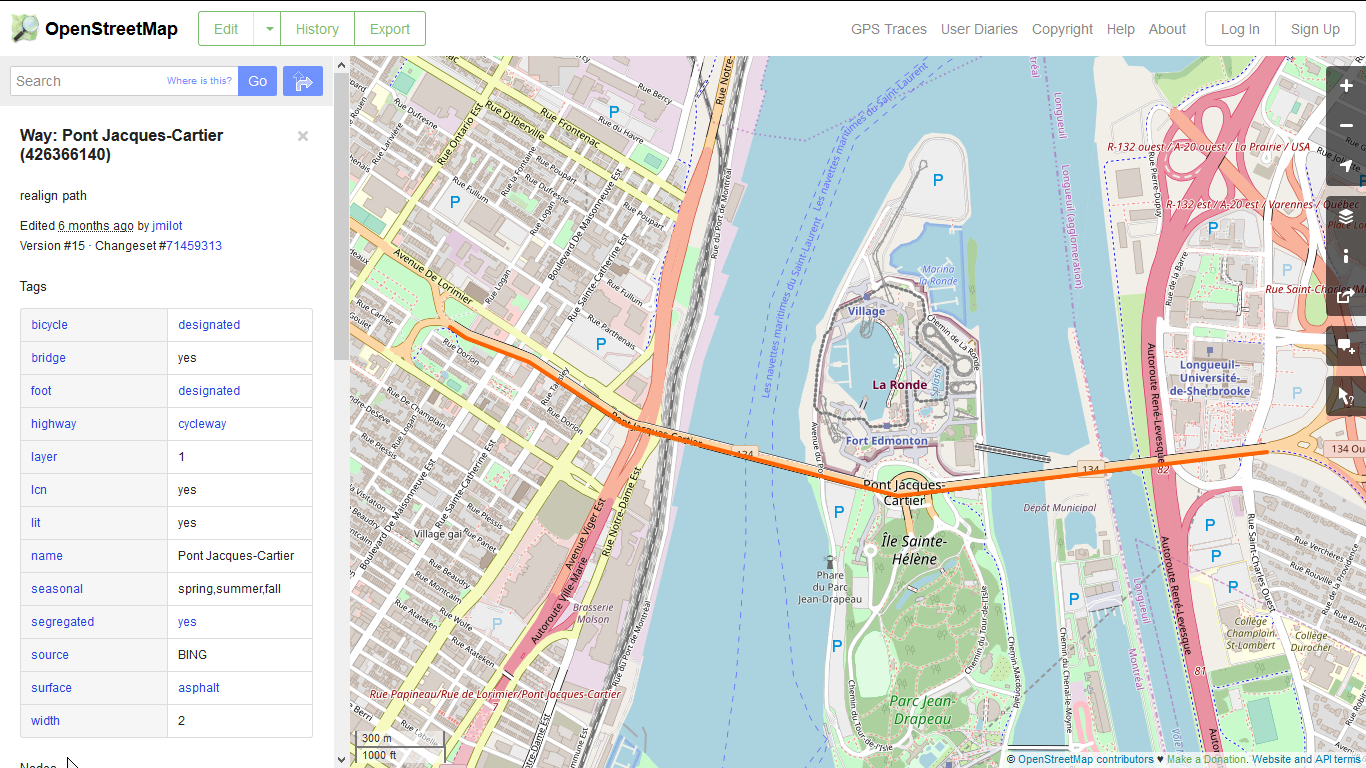
\includegraphics[width=1.0\textwidth]{carte_site_etude}
    \caption{Carte du site d'implantation : le pont cartier et la piste multifonctionnelle en orange sur le pont}
    \label{fig:carte_site_etude}
\end{figure}
